\documentclass[../main.tex]{subfiles}
\graphicspath{{\subfix{../images/}}}


\begin{document}


\subsection{Libraries used for the implementation}

\textit{TensorFlow} is an open-source library created by Google for deep learning applications \cite{TF_2015}. TensorFlow GPU enables TensorFlow to take advantage of the processing power of a GPU, which, inherently speeds up the training process.

\textit{Keras} is a high-level application programming interface (\textit{API}) of TensorFlow written in Python, other deep learning frameworks are available, however, TensorFlow has adopted Keras as the official high-level API making Keras the preferred API. Keras was developed to enable fast development from idea to execution. It was designed to be user friendly to give users a simple method of creating models.

\textit{NumPy} is a library designed with multidimensional arrays in mind and is the preferred library for scientific programming \cite{numpy_2020}. NumPy implements many fundamental mathematical operations as a vectorized alternative, especially when operating on arrays. The reshaping of arrays is another key feature that NumPy implements very well and is vital when dealing with timeseries for RNNs.

\textit{pandas} is an open-source library designed for data manipulation and analysis, and provides a plethora of built-in functions to process data \cite{Pandas_2022}. As the data used for this thesis is stored in csv-files, the choice of \textit{pandas} was clear from the start and further solidified due to the geospatial nature of the data and further on the choice of using GeoPandas.

\textit{Shapely} is an open-source library for Python to manipulate geometric objects. The basic objects are points, lines and polygons.

\textit{Geopandas} is an open-source library that extends \textit{pandas} datatypes and can operate on Shapely objects, and provides vital functions when working with geospatial data \cite{Geopandas_2020}. It is written in Python and allows for almost seamless development between \textit{pandas} and GeoPandas. The library can be quite a challenge to install, especially when other libraries that requires the same libraries are installed or needs to be installed. GeoPandas utilizes \textit{pandas} datatypes to store data and Shapely to operate on the data, for example, coordinates are simply points in a space and areas can be represented as polygons by simply connecting the points with lines. These fundamentals allows the representation and manipulation of geospatial data.

\subsection{Data pre processing}

The years 2009 through 2018 are chosen to train and evaluate the performance of the model. The year 2019 was omitted due to unusual file sizes, which led to the belief that the files for that year are not complete. All these files total approximately 130 gigabytes, which will introduce some limitation on how much of the data is processed at once. The process of finding possible routes in this raw data for further processing and validation involves finding all vessels that have visited the port of interest at any point. Due to the file sizes and amount of data for each file, this process has to be split into smaller chunks of time windows, \textit{i.e.} the number of consecutive months processed at once. With the possibility of vessels starting a route at the end of a month and arriving at the beginning of the next month, larger time windows are preferred, but memory limitations impeded the possibility of very long time windows. Splitting the year into quarters proved to be a good compromise computationally.

The first step involves finding which vessels have visited the port of interest, the port of Naantali, for each month. This step is computationally quite time-consuming, since every row in each file has to be checked, except rows of a previously known vessel. Only once a vessel has been identified to have visited the port of interest it can be skipped, else the row has to be checked. It is impossible to known at what point in time a vessel has visited the port of interest, so every row has to be checked and since a vessel could have made only one visit to the port for the whole period covered, it is unnecessary to store the whole timeline of said vessel for further processing. Rather, only the timeline of when the vessel has visited the port can be fetched, which drastically decreases the required amount of data. The process involves checking each row's latitude and longitude and whether these coordinates are within the bounding box, as seen in Figure \ref{fig:FINLI-box}. This process has to be done once for each file, after which the unique identifiers, \textit{imo}, for every vessel can be stored for future use. Every month can have more than 30 unique vessels, a quarter can have around 80 unique vessels, and the whole timeline is extracted for all vessels for the quarter.

\begin{figure}[H]
	\centering
	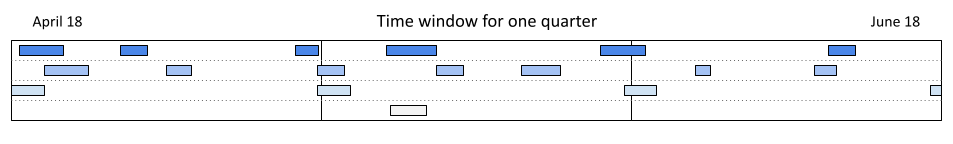
\includegraphics[scale=.45]{timeline.png}
	\caption{Example of one quarter of the year 2018, a \textit{time window}, and from this time window each unique vessel's complete timeline is extracted for further processing. The coloured boxes represent raw AIS data for four unique vessels. Does not represent actual data, rather visualizing the process of finding relevant data in the raw HELCOM dataset.}
	\label{fig:timeline}
\end{figure}

From the complete time window seen in Figure \ref{fig:timeline}, only a fraction of the data is actual viable routes going to the port of interest. Merging the complete time window with AIS data for every vessel generates a timeline for each of the unique vessels discovered in the first step. Within that timeline exists routes going to the port of interest and the next section describes how these routes are extracted and validated.

\subsubsection{Algorithm for extracting routes from dataset}
\label{sec:algo-section}
A route is defined as a series of consecutive AIS messages where the first message in the series is the starting point for a vessel travelling to a port of interest. The last message in the series is the first messages when the vessel has entered the port of interest bounding area, see Figure \ref{fig:FINLI-box}. The routes do not need a specific starting point, as this point bound to any position; rather it will be chosen from one of two possibilities. The end of the route will be the same for all vessels, as the goal is to find all routes coming from somewhere travelling to the port of interest. A good route will also not have any gaps of time during the route.

To find routes coming from anywhere and going to an area of interest or port an iterative approach is used. With a complete historical timeline of one vessel, the routes can be discovered by traversing the timeline in reversed chronological order. The end of a route, \textit{i.e.} the start of the search, is the first point where the vessel is leaving the bounding box. From this position, traversing the timeline, in reversed chronological order, until a predefined condition is met, will give the section of a vessel's timeline which equals a route coming from somewhere travelling to an area of interest.

The condition for when the start of the route, end of the search, is met, is whenever the duration of the route has exceeded 48 hours or the vessel's speed over ground is zero, standing still, for more than 5 consecutive transmitted messages. The 48-hour time limit was defined for the reason that the maximum travel duration in the Baltic Sea is below 48 hours for a vessel moving at the mean speed discovered and vessels travelling from outside the Baltic Sea have reached Kattegat and the edge of the Baltic Sea Area seen in Figure \ref{fig:helcom-area} at this point in time. The reason behind checking that multiple transmitted messages have recorded the speed to be zero is to guarantee that the vessel has actually stopped and not slowed down for other reasons. This condition can still introduce routes that have not started from another port but will minimize these routes.
\\\\
\begin{algorithm}[H]
\SetAlgoNoLine
\SetAlgoNoEnd

\SetKwData{Index}{index}\SetKwData{End}{end}\SetKwData{Start}{start}
\SetKwData{Route}{route}\SetKwArray{R}{R}
\KwIn{DataFrame for one vessel sorted in descending time, a \textit{timeline}}
\KwResult{List \R of all routes found}
\emph{The algorithm searches in reverse order of time from reaching the destination until the start of the route}\;
\BlankLine
\ForEach{row in DataFrame}{
	\Index $\leftarrow$ Keep track of current row\;
	\BlankLine
	\If(\tcp*[f]Only true after finding first route){\Route found}{
		\emph{Start searching from first unknown point}\;
		Skip rows until \Index $=$ \Start\;
	}
	\BlankLine
	\If{current point is in PORT}{
		\ForEach{row in DataFrame starting from \Index}{
			\If(\tcp*[f]Vessel is entering the port){point is outside PORT}{
				\End $\leftarrow$ First point reaching the destination\;
				\BlankLine
				\ForEach{row in DataFrame starting from \End}{
					
					\If{start of route reached}{
						\Start $\leftarrow$ Current row\;
						\R $\leftarrow$ Save route from \End to \Start\;
					}
				}
			}
		}
		\tcc{When a route has been found and saved start search again from the last not visited point.}
	}
}
\caption{Find all routes going to an area of interest}
\label{alg:search}
\end{algorithm}
\vspace*{5mm}

Route validation rules were defined to give an efficient way of discarding any routes that would impact the model's performance and routes that were off no interest for the scope of the thesis.

All routes that did not travel for more than eight hours from start to finish were discarded. The reason for this rule comes from the fact that all vessels will be required to travel through the same area for the final part of the voyage, and the model should perform well in this area, even though these routes are discarded.

A minimum distance travelled rule was used to discard any routes that travelled less than 200 kilometres, that is the total route distance and not how far away from the port the vessel travelled. To navigate out from the port of Naantali and the largest bodies of islands outside of Naantali takes approximately 70 kilometres following the fairway. Moving at 14 knots the time to cover the distance takes just under three hours, however, the speed in this area will most likely be lower for most vessels due to the limited area to manoeuvre.

Any routes that have a time difference between two consecutive AIS messages greater than 12 minutes are also discarded. The reason for this is explained in more detail in Section \ref{sec:timeseries}.

Vessels that have returned to the port of Naantali or are returning to the area around Naantali are also discarded. This combined with the minimum distance travelled required will ensure that, for example, pilot vessels and other leisure vessels will not be in the final training data. Vessels travelling back to the area are not of interest and could impact the model negatively, as these vessels will probably have an abnormal voyage compared to cargo vessels.

Routes that have faulty data, \textit{i.e.} NaN values or other bad values, and which cannot be inferred from the data in any other way are discarded. Examples of this was found where the draught was not recorded only for a small section of the route but could be inferred from the parts where it was recorded. If the values could not be inferred at all, the route was discarded completely.

\begin{figure}[H]
	\centering
	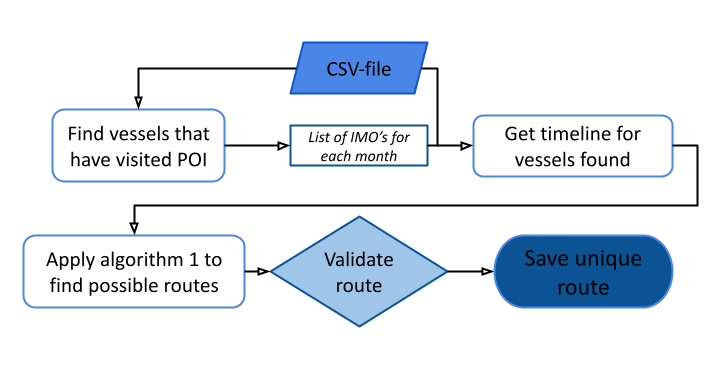
\includegraphics[scale=.5]{data-process.png}
	\caption{Getting routes.}
	\label{fig:flowchart}
\end{figure}

After all of the steps and validations above the final number of routes which fulfil the requirements defined is 3,973. The number of possible candidate routes was 13,955, 70\% of all routes did not meet the requirements and were therefore discarded. This further indicates the issues with the veracity of AIS data. The number of routes that could be possible valid candidates could be higher by generating data for missing gaps on the timeline of the routes, when the gap is below a certain threshold. For the scope of this work, to utilize historical AIS data provided by HELCOM and create a model that can predict the ETA for vessels in the Baltic Sea, the number of routes found does prove it is possible, but with limitations.

\begin{figure}[H]
	\centering
	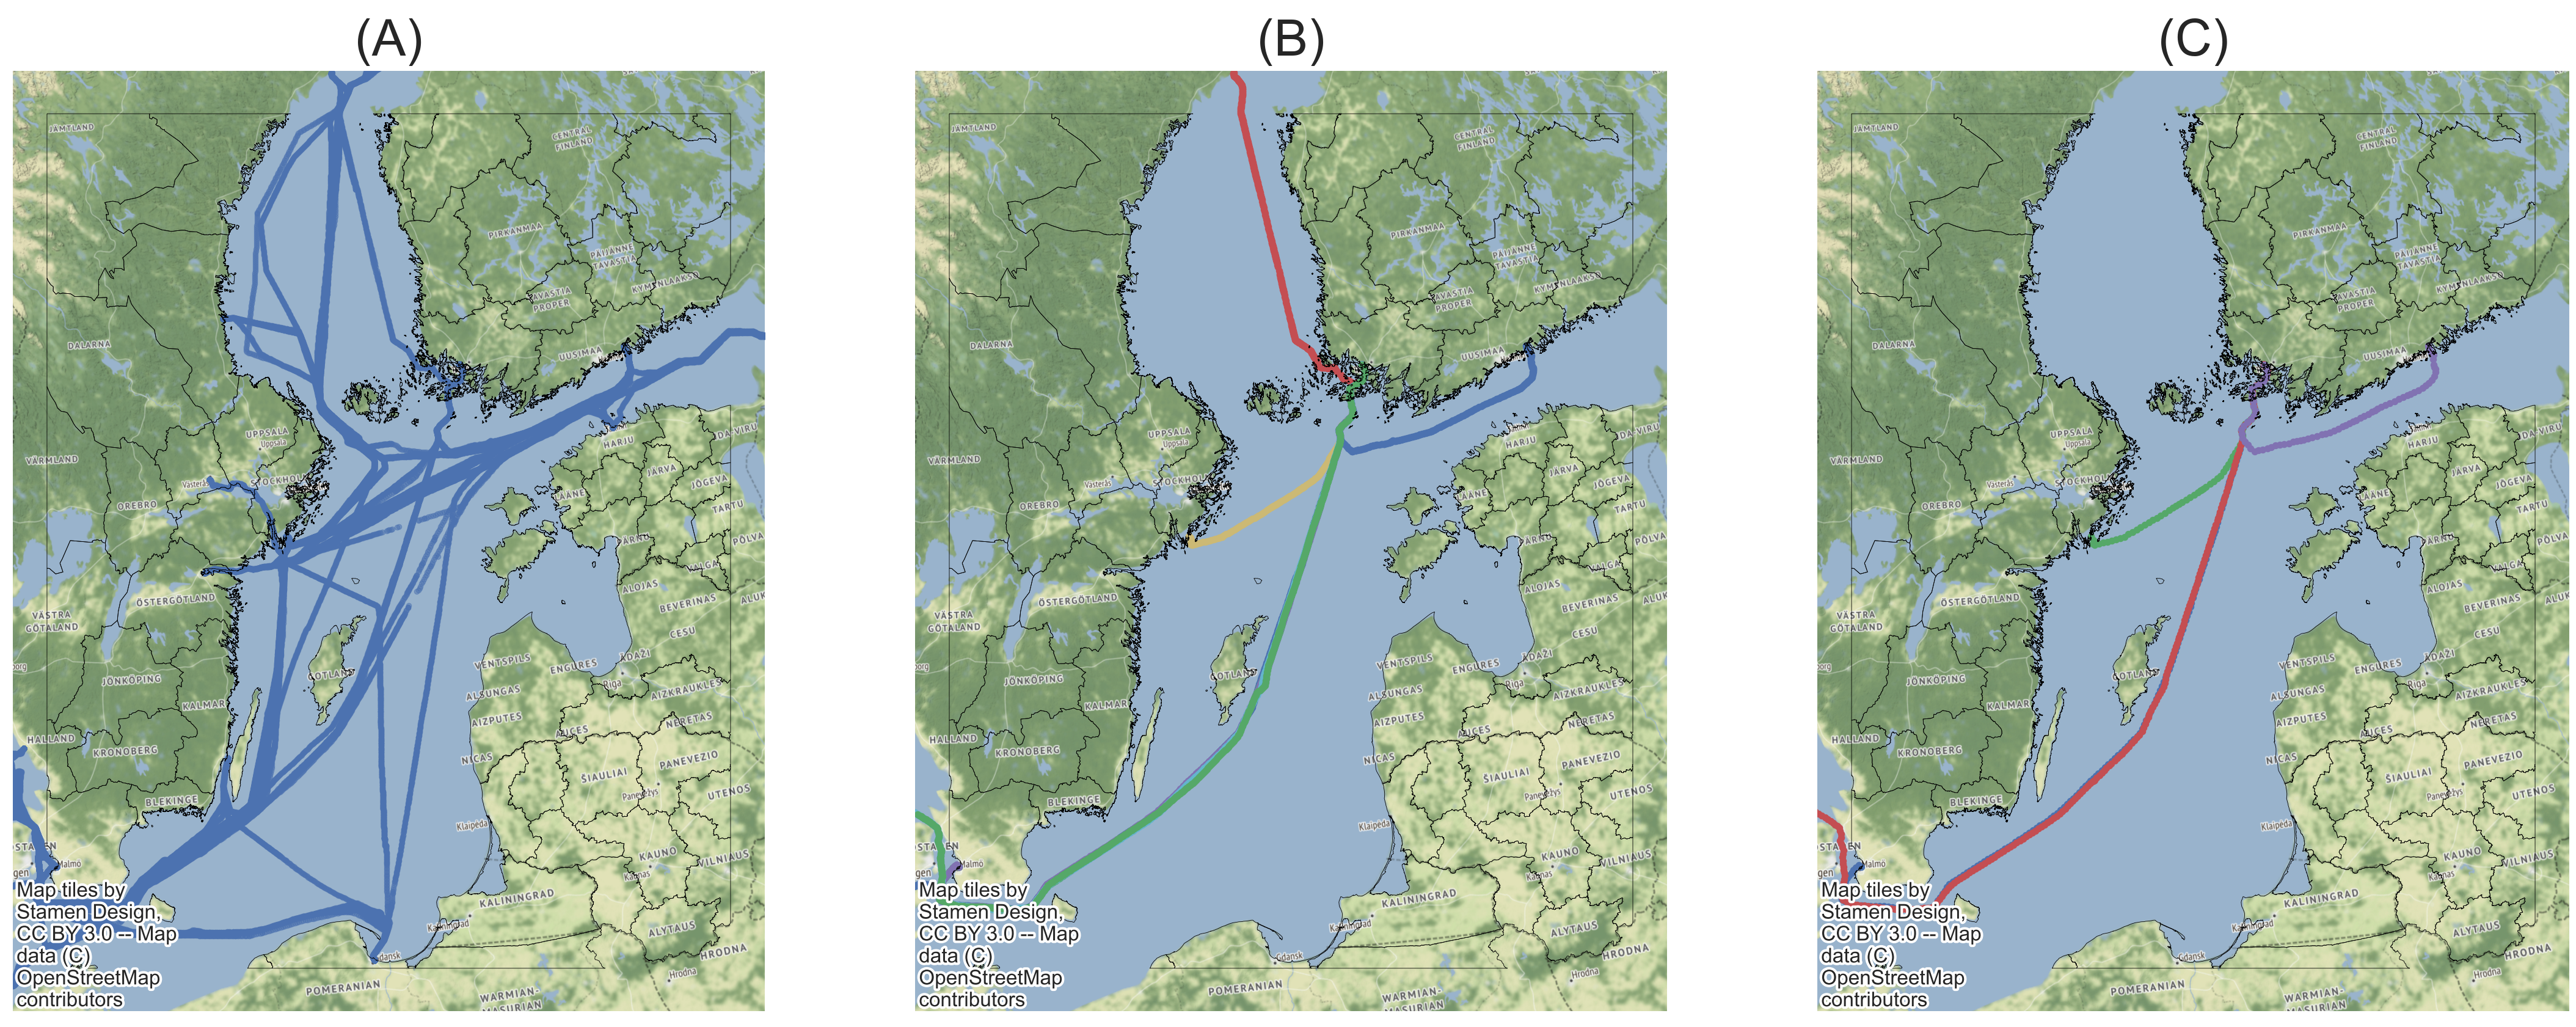
\includegraphics[scale=.45]{route-finding-9256420.png}
	\caption{(A) Complete timeline for one vessel in 2013. (B) All possible routes for the same vessel. (C) All validated routes for one year from one vessel which are used for training. }
	\label{fig:route-finding}
\end{figure}

Figure \ref{fig:route-finding} illustrates these limitations where routes have to be discarded for not meeting the required validation rules. Also with the data in Table \ref{tab:HELCOM-data-percent} in mind, the amount of data of the total timeline that make up the good routes is only a fraction of it.

\subsubsection{Coordinate accuracy}

The latitude and longitudes in the HELCOM dataset have an accuracy of six decimal places, 0.111 metres. This accuracy is not required as the difference in time between a lower accuracy will be within a possible prediction error.

The level of scaling the coordinate accuracy with, was chosen to a decimal degree of three places, that is 0.001 which is 111 meters. The accuracy of the vessel's location will be within approximately 100 meters.

\begin{table}[H]
\centering
\begin{tabular}{|l|c|}
\hline
\rowcolor[HTML]{C0C0C0} 
\textbf{Degrees} & \multicolumn{1}{l|}{\cellcolor[HTML]{C0C0C0}\textbf{Distance}} \\ \hline
1.0              & 111 km                                                         \\ \hline
%\rowcolor[HTML]{EFEFEF} 
0.1              & 11.1 km                                                        \\ \hline
0.01             & 1.11 km                                                        \\ \hline
%\rowcolor[HTML]{EFEFEF} 
0.001            & 111 m                                                          \\ \hline
0.0001           & 11.1 m                                                         \\ \hline
%\rowcolor[HTML]{EFEFEF} 
0.00001          & 1.11 m                                                         \\ \hline
0.000001          & 0.111 m                                                         \\ \hline
\end{tabular}
\caption{Coordinate accuracy by decimal places in decimal degrees for latitude and longitude, from \cite{GIS_2011}}
\label{tab:gis-accuracy}
\end{table}

AIS messages transmitted within approximately 100 metres of each other will be thought of as sent from the same location using this scaling level. With a mean speed for the routes found and used, see Figure \ref{fig:sog-dist}, of approximately 14 knots (25 km/h) and a time difference between messages of 10 minutes a vessel will have moved 2.2 nmi (4.1 km) during this time. With a positional accuracy of approximately 100 metres, this distance can vary but on the open sea a difference in $\pm$ 100 metres does not impact the overall time it will take to reach the destination.


\subsubsection{Feature selection}

The features chosen for training the model on were decided by what is available in the HELCOM dataset, what is possible to infer from available data and what has been proven to be efficient features by previous studies \cite{El_2020, Jahn_2018}.

Most of the features available in the HELCOM dataset were used for the model; latitude and longitude for the position of the vessel at a given point in time, sog to indicate the vessels moving rate, cog for where the vessel's trajectory is heading, draught to indicate the vessel's physical capabilities in combination with the vessel class feature, which is a combination of features, see Figure \ref{fig:vessel-class-def} and, finally, the distance to the destination calculated from the historical route the vessel has taken.

Using the distance left to the destination as a feature does mean that the problem to be solved is, in its simplicity, learning the time it will take to traverse the distance left at the current speed. However, there are many factors that will impact the time it will take to reach the destination which cannot be learned from only the distance to travel and the speed. It is these factors that could be learned by training on historical data and improve the prediction accuracy compared to other simpler solutions.

The target to predict is time to destination (\textit{TTD}) which is in minutes. The TTD prediction is added to the current time and, thus, gives an ETA. The TTD is calculated as the difference between the current time and what time the vessel has arrived at port.

\subsubsection{Time series data windowing and time distribution}
\label{sec:timeseries}

With the routes validated, a final processing step is required to generate the time series data that is fed to the network. Since regular RNN suffers from poor performance when the data are unevenly sampled in terms of time difference between samples, it is vital to normalize the time difference between time steps. The nature of the AIS and the HELCOM dataset means that it is only viable to normalize the sampling interval to a certain degree.

A compromise with the time difference between messages was achieved by as evenly as possible sample data with longer time intervals, discarding messages in that interval, and by this achieving an improved time series with preferable time difference normalization. In this improved time series, the difference between messages is on average at most three minutes. A lower limit of nine minutes was chosen to conform with what was discovered in Section \ref{sec:AIS-stat} and Figure \ref{fig:ais-msg-dist} and the upper bound of twelve minutes has been set when validating the routes. On average, two messages will be discarded, so the time difference is nine minutes. Shorter time intervals should be possible with raw AIS data, but for the dataset used the number of routes that were viable without generating data between messages were too few. Decreasing the longest allowable gap between AIS messages in a route discarded too many routes, \textit{i.e.} a route with at any point a time difference between messages smaller than twelve minutes would have been rejected.

\begin{figure}[H]
	\centering
	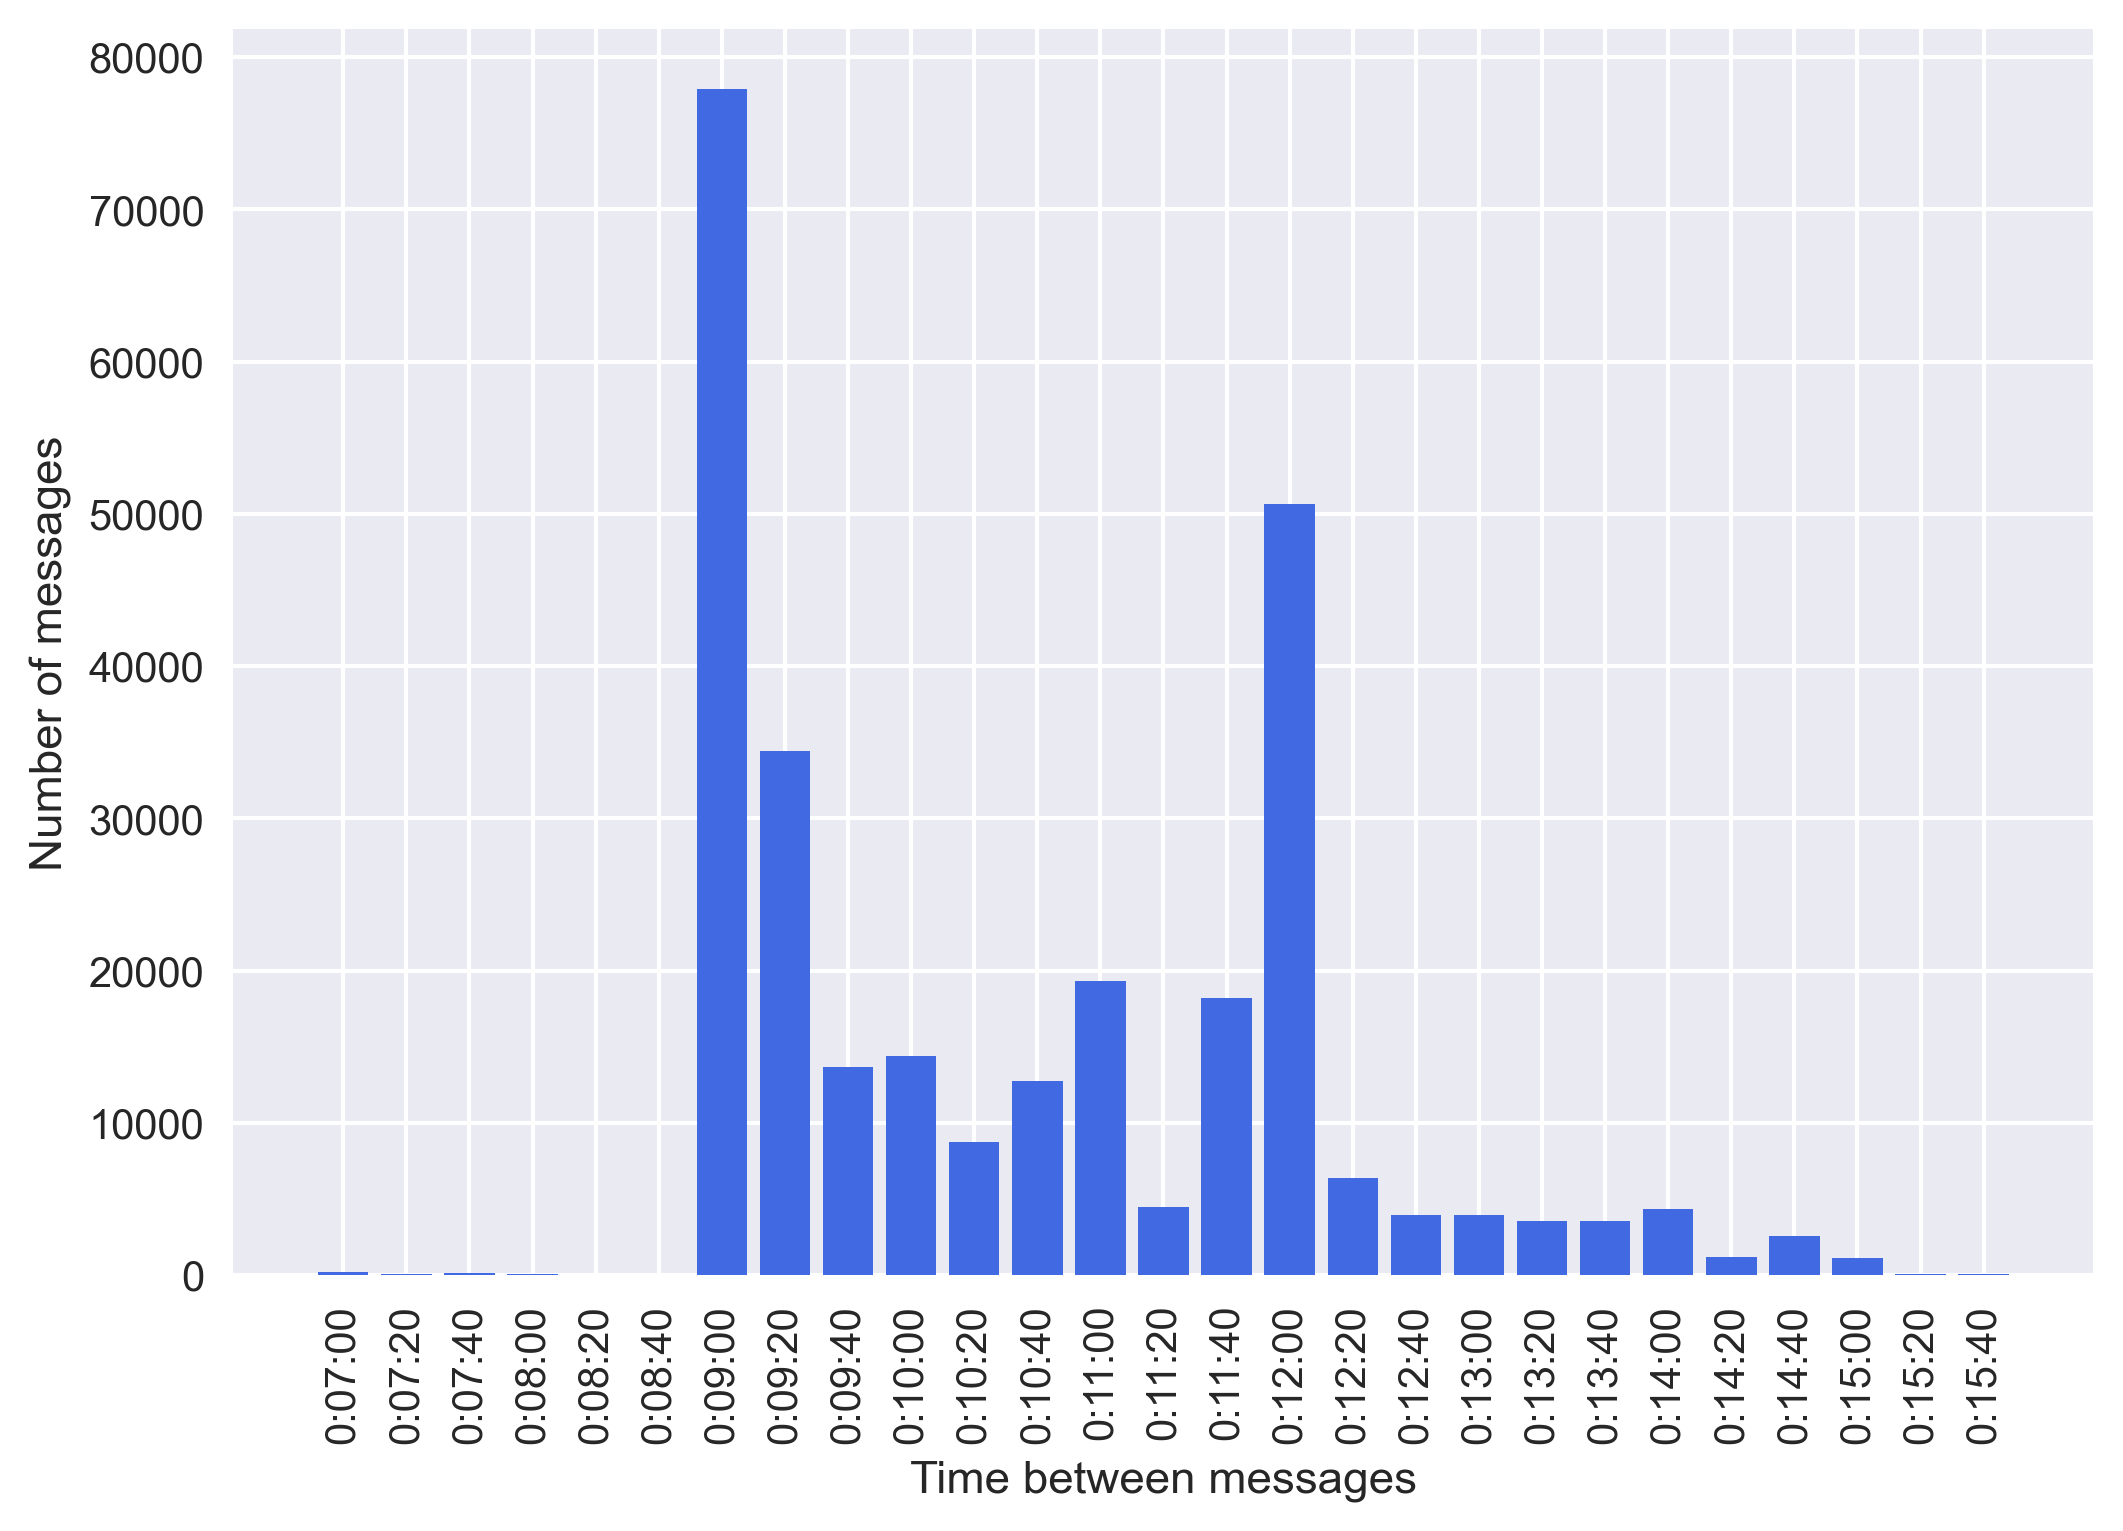
\includegraphics[scale=.6]{2009-2018-routes-message-dist.png}
	\caption{The distribution of time differences between messages for the normalized routes.}
	\label{fig:norm-time}
\end{figure}

In Figure \ref{fig:norm-time}, the normalized time differences are in the range from nine to twelve minutes, with only some exceptions that have a time difference shorter than or longer than this range. The exceptions are for the most part due to the inconsistencies in the recorded time intervals, \textit{e.g.} given one message at time zero $t_0$ with the following messages at $t_{+4}$, $t_{+4}$ and $t_{+7}$ (minutes from the previous message), the first two messages will not be more than nine minutes from the first and the third message will therefore be chosen as the next point in time, with a 15-minute difference. 

\begin{figure}[H]
	\centering
	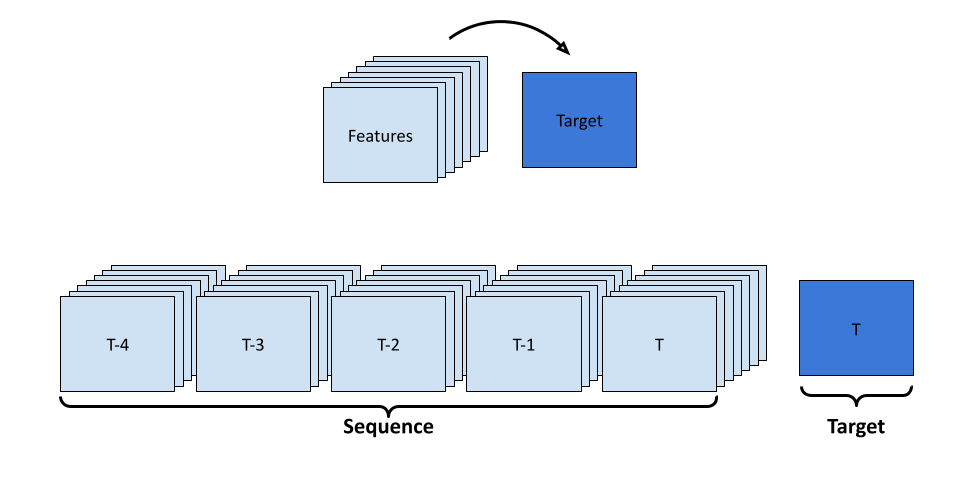
\includegraphics[scale=.4]{sequenced-data.png}
	\caption{Time series sequenced data, with a time window width of five. Each timestep in the sequence has a time difference in the range defined.}
	\label{fig:seq-data}
\end{figure}

With a route consisting of AIS messages with a time difference distribution in the range mentioned above, a time window of $n$ timesteps is generated for the whole route. A time window is defined as $n$ number of consecutive timesteps that create a window of time for the route. Each timestep in this time window consists of all chosen features and the target TTD. For all but the last timestep, the target is discarded and only the final timestep's target is set as the target to predict. Sliding the time window over the whole route, one timestep at a time generates a set of windows that each covers $n$ timesteps. 

\begin{figure}[H]
	\centering
	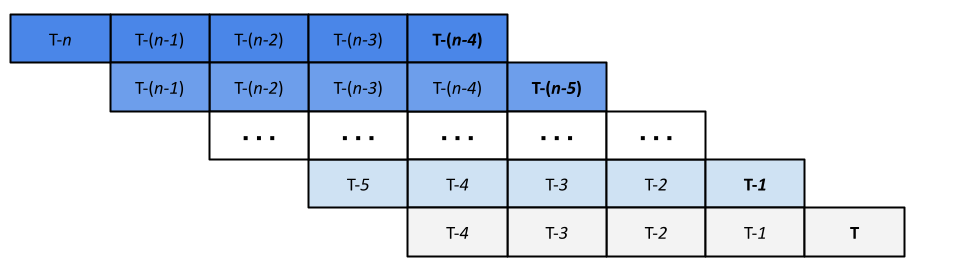
\includegraphics[scale=.4]{time-window.png}
	\caption{Sliding time window for a complete route starting from the end at $T-n$ and ending at the last timestep $T$. A prediction will be made for every last timestep in the time window, marked with bold.}
	\label{fig:time-window}
\end{figure}

A prediction will be made for the last timestep in the time window, which in terms of real-time prediction will require that for the first four timesteps, AIS messages received, a prediction cannot yet be made. After the fifth message a prediction can be made. This also means that any five historical AIS messages could be used, if they fulfil the requirements for the time window.


\subsection{RNN model implementation}
The neural network architecture implemented is a RNN with LSTM units. Earlier work has concluded that that the LSTM unit performed better than other alternatives, in a similar task of predicting the ETA \cite{El_2020}. The decision to not look into other alternatives was supported by these findings and the nature of how RNNs work, compared to regular feedforward neural networks or other types of neural networks.

Keras implements this architecture without much effort required from the user, the main work was put into manipulating and reshaping of the data, as the model requires a certain kind of data structure.

The final model used for training and testing consists of one input layer, two hidden layers and one output layer. During the development stages, single-layer networks and multi-layer networks were compared to each other, and the multi-layer networks performed better every time. 

The input layer takes a vector of shape number of timesteps per time window $t$ and the number of features per timestep $f$. This is the idea behind RNNs capabilities to utilize multiple timesteps in a sequence to predict an output, it takes multiple historical samples and learns the impact of previous samples on the final output.

The two hidden layers consists of 16 cells each and the first hidden layer has the argument \texttt{return\_sequences} set to true, which is required when dealing with deep RNNs. The last hidden layer simply outputs the result of the layer to a single dense cell that outputs the prediction, TTD. The reason for 16 cells in each hidden layer is arbitrary, and while testing the impact of changing the model architecture, it was discovered that the performance difference was negligible between models with the same number of hidden layers but different number of cells.

The model was otherwise left unchanged from the default implementation, \textit{i.e.} the activation was $\tanh$, recurrent activation was sigmoid, recurrent dropout was 0, unroll was false and it uses a bias vector, these settings can be found on \url{https://www.tensorflow.org/api_docs/python/tf/keras/layers/LSTM}. These settings were mostly chosen to utilize the cuDNN implementation, leveraging the GPU accelerated operations.

The optimizer used was the Adam algorithm with defaults settings. The reason for choosing Adam over any of the other available optimizers, was simply due to the performance and the optimizer is thought of, as one of the best performing with RNNs \cite{El_2020, Choi_2019}.


\subsubsection{Phased LSTM}

Comparing the regular LSTM network with a Phased LSTM network, which sould perform better than LSTM when samples are irregularly sampled.


\end{document}